\section{Hardwareentwicklung}
\label{sec:TeilB_Hardware}
In diesem Kapitel wird auf die entwickelte Hardware eingegangen und detailliert dargestellt. Die Abbildungen \ref{fig:teilb_pcb_top} und \ref{fig:teilb_pcb_bot} zeigen die Ober- bzw. Unterseite der 4-Lagigen Platine. In den Bildern sind farblich die einzelnen Bereiche der Platine markiert. 

\begin{table}[h]
\begin{tabular}{|p{8cm}|p{5.5cm}|}\hline
\rowcolor{TableBackgroundColor} 
   \textbf{Bereich auf Platine} & \textbf{Farbe}\\ \hline
  HDMI Eingang &  \textcolor{blue}{Blau} \\ \hline
  RGB Bridge & \textcolor{yellow}{Gelb} \\ \hline
  LVDS Bridge & \textcolor{magenta}{Magenta}  \\ \hline
  EDID-Daten &  \textcolor{orange}{Orange} \\ \hline
  Spannungsversorgung &  \textcolor{green}{Grün} \\ \hline 
\end{tabular}
\caption{Teil B: Farblich gekennzeichnete Bereiche auf der Platine}
\label{tab:pcb_areas}
\end{table}

\begin{figure}[htbp]
        %\begin{center}
        \centering
        \begin{subfigure}[htp]{0.48\textwidth}
                \fbox{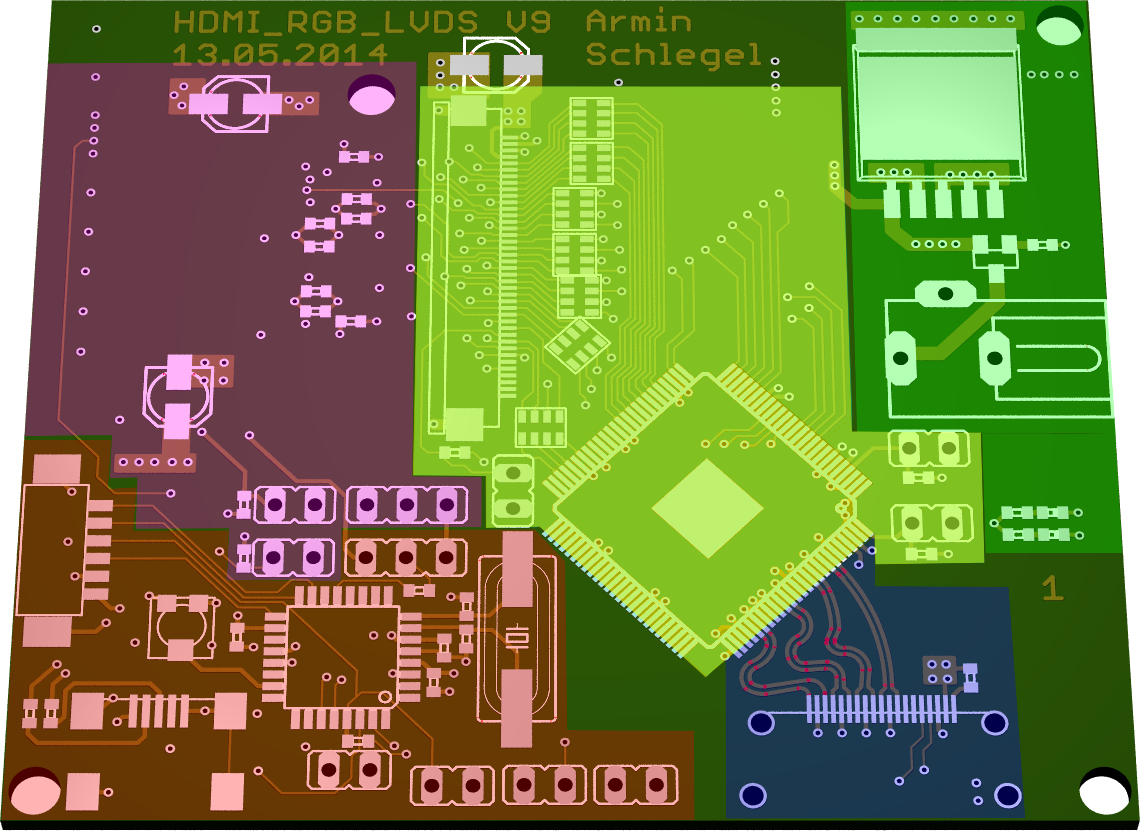
\includegraphics[width=1\textwidth]{TeilB/HDMI_RGB_LVDS_V9_top.png}}
                \caption{Top Layer}
                \label{fig:teilb_pcb_top}
        \end{subfigure}
\quad 
        \begin{subfigure}[htp]{0.48\textwidth}
               \fbox{ 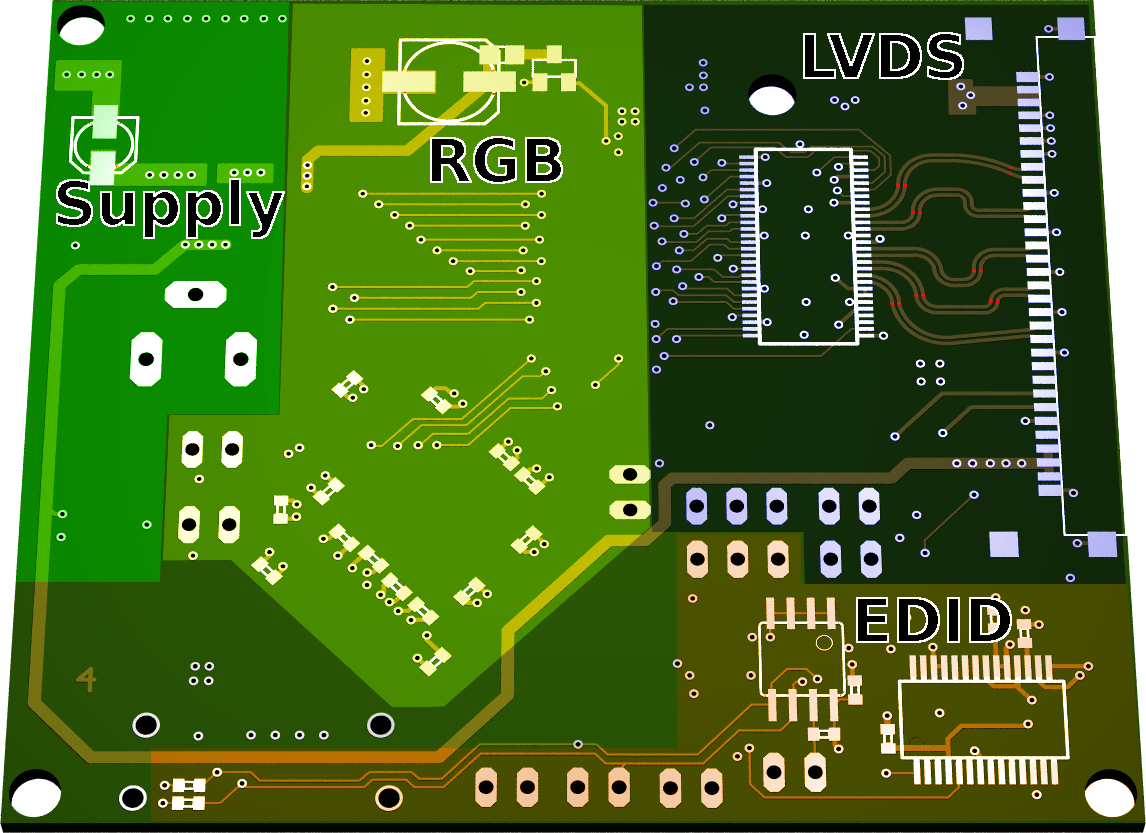
\includegraphics[width=1\textwidth]{TeilB/HDMI_RGB_LVDS_V9_bot.png} }              				\caption{Bottom Layer}
                \label{fig:teilb_pcb_bot}
        \end{subfigure}
		%\end{center}
        \caption{HDMI RGB/LVDS Board}
        \label{fig:teilb_pcb}
\end{figure}

In den folgenden Abschnitten wird auf die Teilbereiche der Platine im Einzelnen eingegangen. 

\subsection{HDMI-Eingang}
Der HDMI-Eingang wird durch eine HDMI-Buchse der Firma \code{FCI} realisiert und wird mittels Impedanzkontrollierten Leitungen an die RGB-Bridge weitergegeben. Diese Leitungen sind mit einer differentielle Impedanz von 100$\Omega$ spezifiziert. Zu beachten ist, dass alle Leitungspaare dieselbe Länge aufweisen, da sonst Laufzeitunterschiede und Fehlabtastung innerhalb der verschiedenen Signalpaare auftreten und zu Fehlern führen können. Die Impedanz der differentieller Leitungen lässt sich nach den Gleichungen 
%
\begin{equation}
Z_0 = \frac{88.75}{\sqrt{\epsilon_r + 1.47}} \cdot ln\left(\frac{5.97 \cdot h}{0.8 \cdot W + t}\right)
\label{equ:z_0}
\end{equation}
%
und
%
\begin{equation}
Z_{Diff} = 2 \cdot Z_0  \cdot \left(1-0.48 \cdot e^{-0.96\frac{s}{h}}\right)
\label{equ:z_diff}
\end{equation}
%
mit den Parametern entsprechend \reft{tab:z_parameter} (siehe \cite{TI2007}). Hier erhält man eine Impedanz $Z_0$ von 128$\Omega$ und eine differentielle Impedanz von 146$\Omega$. Aufgrund der kurzen Leitungslängen von maximal 11mm, spielt diese Fehlanpassung keine große Rolle und kann vernachlässigt werden.
\begin{table}[h]
\begin{tabular}{|p{7cm}|p{3cm}|p{3cm}|}\hline
\rowcolor{TableBackgroundColor} 
   \textbf{Parameter} & \textbf{Bezeichnung} & \textbf{Wert}	\\ \hline
    Dielektrikum 					& $\epsilon_r$	& 4.2		\\ \hline
	Breite der Leitungen  		 	& W 			& 0.28 mm	\\ \hline
	Abstand des Paares zueinander 	& s 			& 0.17 mm 	\\ \hline
	Dicke des Dielektrikums 		& h 			& 1.6 mm 	\\ \hline 
	Dicke der Leiterbahn 			& t 			& 35 µm		\\ \hline 
\end{tabular}
\caption{Teil B: Parameter bezüglich Impedanz der HDMI-Leitungen}
\label{tab:z_parameter}
\end{table}
\refa{fig:hdmi_leitungen} zeigt die TDMS-Leitungspaare, bei der der gleichmäßige Abstand zwischen den Leitungen einzelner Paare, sowie die gleiche Länge der Paare selbst eingehalten wird. 
\begin{figure}[htp]
%\begin{minipage}[t]{0.8\textwidth}
%\begin{figure}[h]
	\centering
\fbox{	\includegraphics[width=0.6\textwidth]{TeilB/hdmi_stecker.png}}
	\caption{Teil B: HDMI Leitungen}
	\label{fig:hdmi_leitungen}
\end{figure}
Neben den eigentlichen Video-Signalen befinden sich noch die $I^2C$-Signale \code{SCL} und \code{SDA} des EDID-EEPROMs sowie eine Hot-Plug-Detection auf der HDMI-Buchse.

\subsection{RGB-Bridge}


\subsection{LVDS-Bridge}
\subsection{EDID-Daten}
\subsection{Spannungsversorgung}
